
\iffalse 
Assignment 6a
Date    : 11th May 2021
Course  : Applied Programming Lab(EE2703)
Faculty : Prof. Harishankar Ramachandhran

Submission by : Santosh G (EE19B055)

To compile and get the Report(PDF):
1) python3 EE2703_ASSIGN6A_EE19B055.py  (Atleast Once, for the plots)
2) pdflatex EE2703_ASSIGN6A_EE19B055.tex
 
PS: Run "EE2703_ASSIGN6A_EE19B055.py" using the above command atleast once before running this code, as this program needs the plots.
\fi
\documentclass[11pt, a4paper]{article}
\usepackage{graphicx}
\usepackage{amsmath}
\usepackage[margin=0.6in]{geometry}
\usepackage{listings}
\usepackage{float}

\title{APL(EE2703): Simulations(Assignment 6A)} % Title
\author{Santosh G  (EE19B055)} % Author name
\date{\today} % Date for the report

\begin{document}
    \maketitle % Insert the title, author and date

    \section{Aim of the Assignment:}   %Introduction to the assignment
        \begin{itemize}
            \item Simulate an 1-D tubelight using python.
            \item Analyze the the movement of electons and the emissions they make.
        \end{itemize}
        This shall be achieved by assigning initial values and updating the values continuously
    \section{Introduction}
    Python is very helpful for simulating models. We use a 1-D model of a tubelight.A uniform electric field is present which accelerates electrons. Electrons are emitted by the cathode with zero energy, and accelerate in this field. When the energy crosses a threshold energy $E_0$, they can drive atoms to excited states. The relaxation of these atoms results in light emission. Electrons reaching the anode are absorbed and lost. Each “time step”, an average of N electrons are introduced at the cathode.
       
        \section{Simulation}
            \begin{itemize}
	    \item
	    A sumlation is created where a 1-D tubelight is assumed, which is divided into "n" sections. After every time instant, "M" electrons are injected. The simulations are run for "nk" times. 
	    \item
	    The electrons have the potential to excite only after the atoms reach a velocity of "u0". Beyond this velocity, there is a probability p in each turn that a collision will occur and an atom excited. The excited electron’s velocity reduces to zero if it collides.
	    \item
	    We need to collect information of the particles and update them after every turn which is being done in the follwing bolck of code.
	    \item
	    The block of code, performing iterations:
	    \end{itemize}
    
    
	\lstinputlisting[language=Python,firstline=39,lastline=102]{EE2703_ASSIGN6A_EE19B055.py}
        
        \section{Plots}
	From the collected data, the following plots are made:\\
	\begin{itemize}
	\item
	
	Electron Density Histogram:
	The denisty(availablity) of electrons are plotted against the location they are found at.
             \begin{figure}[H]
                    \centering
                    \setlength\tabcolsep{2pt}
                    \begin{tabular}{cc}
                       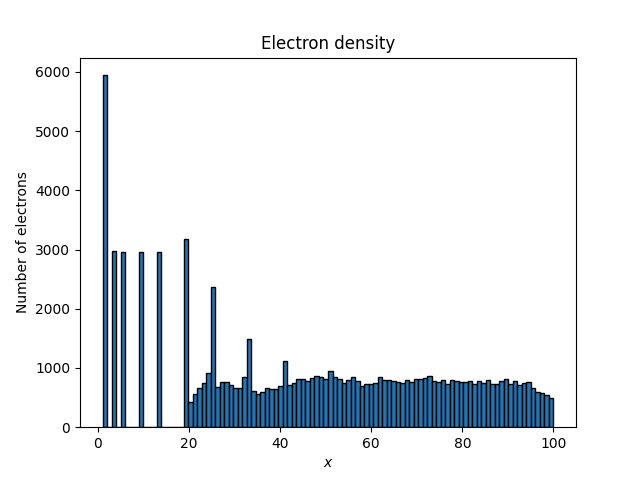
\includegraphics[scale=0.9]{Figure 1.png}
                    \end{tabular}
                    \caption{Electon Density Histogram} 
                \end{figure}
                
 	\item	
	 Emission Intensity Histogram:
	 \\The intensity of emissions made by atoms are plotted against the location of emission
	 \\Some of the data that is being used to plot the following diagram is printed below.
	 
        \lstinputlisting[firstline=1,lastline=20]{data.txt} 
	 
             \begin{figure}[H]
                    \centering
                    \setlength\tabcolsep{2pt}
                    \begin{tabular}{cc}
                       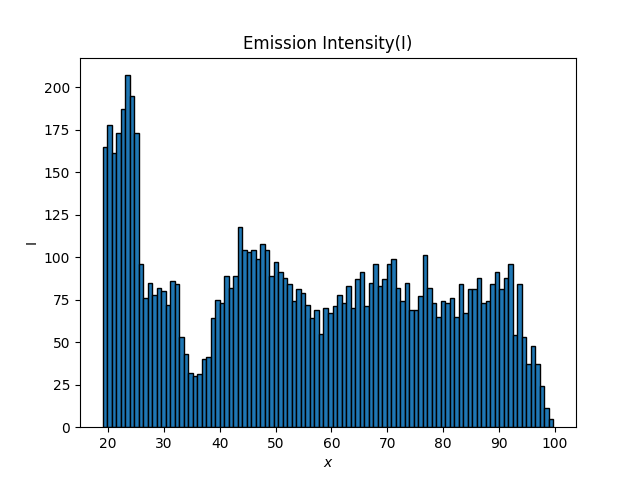
\includegraphics[scale=0.9]{Figure 2.png}
                    \end{tabular}
                    \caption{Emission Intensity Histogram} 
                \end{figure}
                
        \item
        Electron Phase space diagram:
        \\The velocity of the electons are plotted against the locations
		\begin{figure}[H]
			\centering
			\setlength\tabcolsep{2pt}
			\begin{tabular}{cc}
			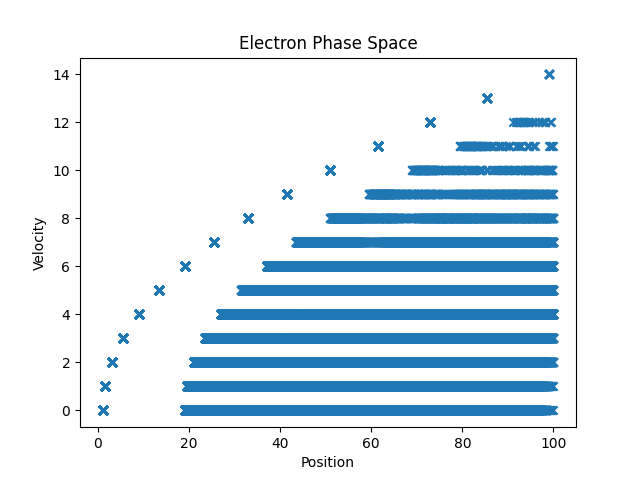
\includegraphics[scale=0.9]{Figure 3.png}
			\end{tabular}
			\caption{Phase Space Diagram} 
                \end{figure}
        \end{itemize}
        
    \section{Conclusion}
    \begin{itemize}
    \item
    Electrons get excited due to electric field, start gaining velocity and hence move around.
    
    \item
    The same happens with other electrons and electrons start to collide with each other and other atoms, leading to exchange of energy.
    
    \item
    Most of the current passes through bottom side of the plate as there is complete path for current to flow unlike the other sides of the plate.
    \item
    These energy excitations and de-excitation causes emissions, giving out light. 
    
    \end{itemize}    
\end{document}
